\documentclass{standalone}
\usepackage{tikz}
\usepackage{ctex,siunitx}
\setCJKmainfont{Noto Serif CJK SC}
\usepackage{tkz-euclide}
\usepackage{amsmath}
\usetikzlibrary{patterns, calc,3d}
\usetikzlibrary{decorations.pathmorphing,decorations.pathreplacing,decorations.shapes}
\begin{document}
\small
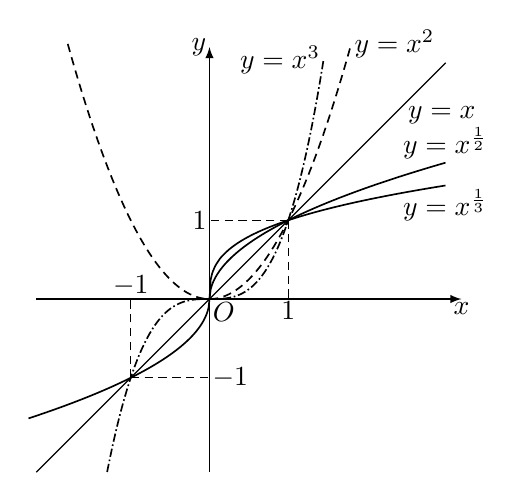
\begin{tikzpicture}[>=latex,scale=1.0,inner sep=1pt]
  \draw[->](-2.2,0)--(3.2,0)node[below]{$x$};
  \draw[->](0,-2.2)--(0,3.2)node[left]{$y$};
  \node at (0,0)[below right]{$O$};
  \draw[semithick,samples=200,domain=0:3.0]plot(\x,{sqrt(\x)})node[above]{$y=x^{\frac12}$};
  \draw[semithick,samples=200,domain=0:2.3]plot(-\x,{-sqrt(\x)});
  \draw[semithick,samples=200,domain=0:3.0]plot(\x,{pow(\x,1/3)})node[below]{$y=x^{\frac13}$};
  \draw[semithick,densely dashed,samples=200,domain=-1.8:1.8]plot(\x,\x*\x)node[right]{$y=x^2$};
  \draw[semithick,densely dashdotted,samples=200,domain=-1.3:1.45]plot(\x,\x*\x*\x)node[left]{$y=x^3$};
  \draw(-2.2,-2.2)--(3,3)node[pos=0.9,below right]{$y=x$};
  \draw[very thin,densely dashed](1,1)--(1,0)node[below]{$1$};
  \draw[very thin,densely dashed](1,1)--(0,1)node[left]{$1$};
  \draw[very thin,densely dashed](-1,-1)--(0,-1)node[right]{$-1$};
  \draw[very thin,densely dashed](-1,-1)--(-1,0)node[above]{$-1$};
\end{tikzpicture}
\end{document}